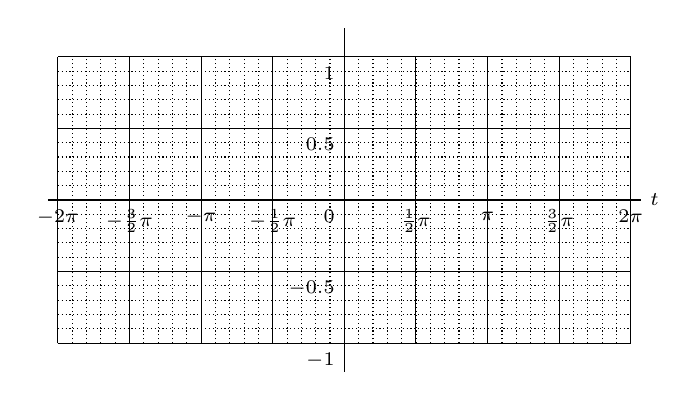
\begin{tikzpicture}[xscale=0.579, yscale=1.818]
	\def\piv{3.1416}
	\coordinate (o) at (0,0);
	\draw (o) ++(-6.5,0) -- ++(13, 0) node [anchor=west] {\scriptsize $t$};
	\draw (o) ++(0,-1.2) -- ++(0, 2.4);% node [anchor=south] {\scriptsize $x(t)$};	
	
	\foreach \y in {-1, -0.9, ..., 1}
	{
		\draw[thin, densely dotted] (-2*\piv, \y) -- ++(4*\piv, 0);
	}	

	\foreach \x in {- 6.2832, -5.9690, ...,  6.2832}
	{
		\draw[thin, densely dotted]  (\x, -1) -- ++(0,2);
	}		
	
	
	\foreach \x/\v in {-2*\piv/-2, -1.5*\piv/-\frac{3}{2}, -1*\piv/-, -0.5*pi/{-\frac{1}{2}},  0.5*\piv/\frac{1}{2}, 1*\piv/, 1.5*\piv/\frac{3}{2}, 2*\piv/2}
	{
		\draw (\x, -1) -- ++(0,2);
		\node at (\x, 0) [anchor=north, minimum height=0.4cm] {\scriptsize $ \v\pi$};
	}
	\foreach \y in {-1, -0.5, 0, 0.5, 1}
	{
		\draw (-2*\piv, \y) -- ++(4*\piv, 0);
		\node  at (0, \y) [anchor=north east] {\scriptsize $ \y $};
	}

\end{tikzpicture} 